\documentclass[9pt, landscape, a4paper]{article}

\usepackage{fontspec}
\renewcommand{\normalsize}{\fontsize{9}{11}\selectfont}
\usepackage[english]{babel}
\babelfont{rm}{Noto Sans}
\babelfont{sf}{Noto Sans}

\usepackage{amsmath}
\usepackage{amssymb}
\usepackage{hyperref}
\usepackage{url}
\usepackage{graphicx}
\usepackage{geometry}
\usepackage{enumitem}
\usepackage{parskip}
\usepackage{chemfig}
\usepackage{pdfpages}
\usepackage{eso-pic}
\usepackage{xcolor}
\usepackage{tikz}
\usepackage{fancybox}
\usepackage{makecell}
\usepackage{pgfplots}
\usepackage{ulem}
\usepackage{wrapfig}
\usepackage{subcaption}
\usepackage{esvect}
\usepackage{siunitx}
\usepackage{mathtools}
\usepackage{varwidth}
\usepackage{multicol}
\usepackage{titlesec}
\usepackage{bm}
\usepackage{forest}
\usepackage{upgreek}
\usepackage{tabularx}
\usepackage{booktabs}
\usepackage{colortbl}
\usepackage[column=O]{cellspace}
\usepackage{tcolorbox}
\usepackage{fancyhdr}
\usepackage{cancel}

\usetikzlibrary{arrows, arrows.meta}
\usetikzlibrary{decorations.pathreplacing}
\usetikzlibrary{decorations.markings}
\usetikzlibrary{patterns}
\pgfplotsset{compat=1.18}

\definecolor{darkgreen}{rgb}{0.0, 0.6, 0.0}
\DeclareMathOperator\arctanh{arctanh}

% ============= TABLE COLORS =============
\definecolor{col1}{RGB}{80,60,160}
\definecolor{col2}{RGB}{40,140,60}
\definecolor{col3}{RGB}{50,80,180}
\definecolor{col4}{RGB}{200,100,0}
\definecolor{headerblue}{RGB}{220,230,245}
\definecolor{headertxt}{RGB}{40,60,120}
\definecolor{notebg}{RGB}{255,248,220}
\definecolor{noteborder}{RGB}{200,160,0}

% ============= GEOMETRY =============
\geometry{
  a4paper,
  landscape,
  left=0.5cm,
  right=0.5cm,
  top=1.5cm,
  bottom=0cm,
  footskip=0cm
}

\setlist{nosep, leftmargin=*}

\AtBeginDocument{
  \setlength{\abovedisplayskip}{3pt}
  \setlength{\belowdisplayskip}{3pt}
  \setlength{\abovedisplayshortskip}{0pt}
  \setlength{\belowdisplayshortskip}{0pt}
}

% ============= HEADER & TITLES =============
\pagestyle{fancy}
\fancyhf{}
\rhead{\small \vspace*{.1cm}Electrical Power Grid Cheatsheet}
\lhead{\small \vspace*{.1cm}Matteo Frongillo}
\cfoot{\small \thepage/10}
\renewcommand{\headrulewidth}{0pt}
\setlength{\headsep}{4pt}

\titlespacing*{\part}{0pt}{2pt}{1pt}
\titlespacing*{\section}{0pt}{2pt}{1pt}
\titlespacing*{\subsection}{0pt}{2pt}{1pt}
\titlespacing*{\subsubsection}{0pt}{1pt}{1pt}

\titleformat{\part}{\large\bfseries\color{black}}{}{0em}{}
\titleformat{\section}{\normalsize\bfseries\color{red!80}}{}{0em}{}
\titleformat{\subsection}{\footnotesize\bfseries\color[HTML]{007AFF}}{}{0em}{}
\titleformat{\subsubsection}{\footnotesize\bfseries\color[HTML]{007355}}{}{0em}{}

% ============= META DATA =============
\newcommand{\pdftitle}[1]{\hypersetup{
  colorlinks=true,
  linkcolor=black,
  urlcolor=blue,
  pdftitle={#1},
  pdfauthor={Matteo Frongillo}
}}

% ============= RENEW COMMANDS =============
\makeatletter
\renewcommand{\author}[1]{%
  \def\@author{%
    #1\\
    \parbox{\textwidth}{%
      \centering
      \small Last update: \today
    }
  }%
}
\makeatother

\let\emptyset\varnothing

\makeatletter
\pgfmathdeclarefunction{arctan}{1}{%
  \begingroup
  \pgfmathparse{rad(atan(#1))}%
  \endgroup
}
\makeatother

\renewcommand{\tau}{\uptau}
\renewcommand{\nu}{\upnu}
\let\mathto\to
\renewcommand{\to}{\ensuremath{\mathto}\ }
\renewcommand{\Im}{\mathrm{Im}}
\renewcommand{\Re}{\mathrm{Re}}

\renewcommand{\CancelColor}{\color{red}}

% ============= NEW COMMANDS =============
\newtcolorbox{exercisebox}[1][Exercise]{
  colback=gray!5,
  colframe=gray!75!black,
  coltitle=white,
  colbacktitle=gray!75!black,
  title={\footnotesize\textbf{#1}},
  fontupper=\footnotesize,
  boxrule=0.6pt,
  arc=2pt,
  left=4pt,
  right=4pt,
  top=3pt,
  bottom=3pt
}

\newcommand{\figbox}[1]{
  \begin{center}
    \fbox{\begin{varwidth}{\textwidth} #1 \end{varwidth}}
  \end{center}
}

\newcommand{\wrapfill}{
  \par
  \ifnum \value{WF@wrappedlines} > 0
    \addtocounter{WF@wrappedlines}{-1}%
    \null\vspace{
      \arabic{WF@wrappedlines}
      \baselineskip
    }
    \WFclear
  \fi
  \phantom{}
}

\ExplSyntaxOn
\DeclareDocumentCommand{\integral}{d[] d[] d[] d[]}
{
  \IfNoValueTF{#3}{
    \IfNoValueTF{#4}{
      \displaystyle \int #1\,d#2
    }{
      \text{Error: either 2 or 4 arguments must be provided}
    }
  }{
    \IfNoValueTF{#4}{
      \text{Error: either 2 or 4 arguments must be provided}
    }{
      \displaystyle
      \int\limits
      \IfNoValueF{#1}{\c_math_subscript_token{#1}}
      ^{\IfNoValueTF{#2}{}{#2}}
      #3\, d#4
    }
  }
}
\ExplSyntaxOff

\newcommand*\circled[1]{\tikz[baseline=(char.base)]{
  \node[shape=circle,draw,inner sep=1pt] (char) {\small #1};}}

\makeatletter
\newcommand*{\rom}[1]{\expandafter\@slowromancap\romannumeral #1@}
\makeatother

\makeatletter
\newcommand{\shorteq}{\mathrel{\mkern0.2mu\mathpalette\shorteq@\relax\mkern0.2mu}}
\newcommand{\shorteq@}[2]{\scalebox{0.5}[1]{$\m@th#1=$}}

\newcommand{\longeq}[1]{\mathrel{\mathpalette\longeq@{#1}}}
\newcommand{\longeq@}[2]{%
  \begingroup
  \sbox\z@{$\m@th#1=$}%
  \ifdim#2<\wd\z@
    \resizebox{#2}{\height}{\box\z@}%
  \else
    \ifdim#2<3\wd\z@
      \hbox to #2{$\m@th#1=\hss=\hss=\hss=$}%
    \else
      \hbox to #2{$\m@th#1=\cleaders\hbox to 0.2\wd\z@{\hss$#1=$\hss}\hfil=$}%
    \fi
  \fi
  \endgroup
}
\makeatother

\newcommand{\const}{%
  \ \mathrel{\ooalign{%
    \hfil$c$\hfil\cr
    \hfil\kern0.10em\raisebox{-0.4ex}{\rule{0.08pt}{1.7ex}}\hfil\cr
  }}%
}

\makeatletter
\define@key{Gin}{lw}[1]{\setkeys{Gin}{width=#1\linewidth}}
\newcommand{\lw}{lw}
\makeatother

\newcommand{\difference}{\,\backslash\,}
\newcommand{\rem}{\underline{Remark}: }
\newcommand{\nots}{\underline{Notation}: }
\newcommand{\note}{\underline{Note}: }
\newcommand{\prf}{\underline{Proof}: }
\newcommand{\exs}{\underline{Example}: }
\newcommand{\defs}{\underline{Definition}: }
\newcommand{\wrn}{\underline{Warning}: }
\newcommand{\sht}{\ |\ }
\newcommand{\pph}[1]{\paragraph{#1} \phantom{}\\}
\newcommand{\dm}{\displaystyle}
\newcommand{\rad}{^{\mathrm{c}}}
\newcommand{\dsum}[2]{\displaystyle \sum_{#1}^{#2}}
\newcommand{\dx}[2]{\dfrac{{\mathrm{d}}^{#1}{#2}}{\mathrm{d}x^{#1}}}
\newcommand{\der}[2]{\dfrac{{\mathrm{d}}{#1}}{\mathrm{d}{#2}}}
\newcommand{\cel}{\ensuremath{^\circ}C}
\newcommand{\todo}{{\color{red}TODO}}
\newcommand{\hr}{\vspace{0.1cm}\par\vspace{-.5\ht\strutbox}\noindent\rule{\linewidth}{.5pt}\par\vspace{0.1cm}}

\DeclareMathOperator{\rot}{rot}

% ============= DOCUMENT CONTENT =============
\begin{document}
\pdftitle{Electrical Power Grid}

\setlength{\columnsep}{0.5cm}
\begin{multicols*}{3}
\raggedcolumns

\footnotesize
\vspace*{-.5cm}
\part{Exercises -- Power grid}
\textbf{Exercise 1: Power-flow sign convention}\\
\underline{Data}:
\begin{gather*}
  \underline{U}_1 = 76 \angle 4^\circ\,\mathrm{kV}, \qquad
  \underline{U}_2 = 76 \angle 8^\circ\,\mathrm{kV}, \qquad
  \underline{U}_3 = 76 \angle -11^\circ\,\mathrm{kV},\\
  \underline{I}_{12} = 450 \angle -15^\circ\,\mathrm{A}, \qquad
  \underline{I}_{31} = 300 \angle 18^\circ\,\mathrm{A}, \qquad
  \underline{I}_{32} = 500 \angle -11^\circ\,\mathrm{A}
\end{gather*}
\begin{center}
  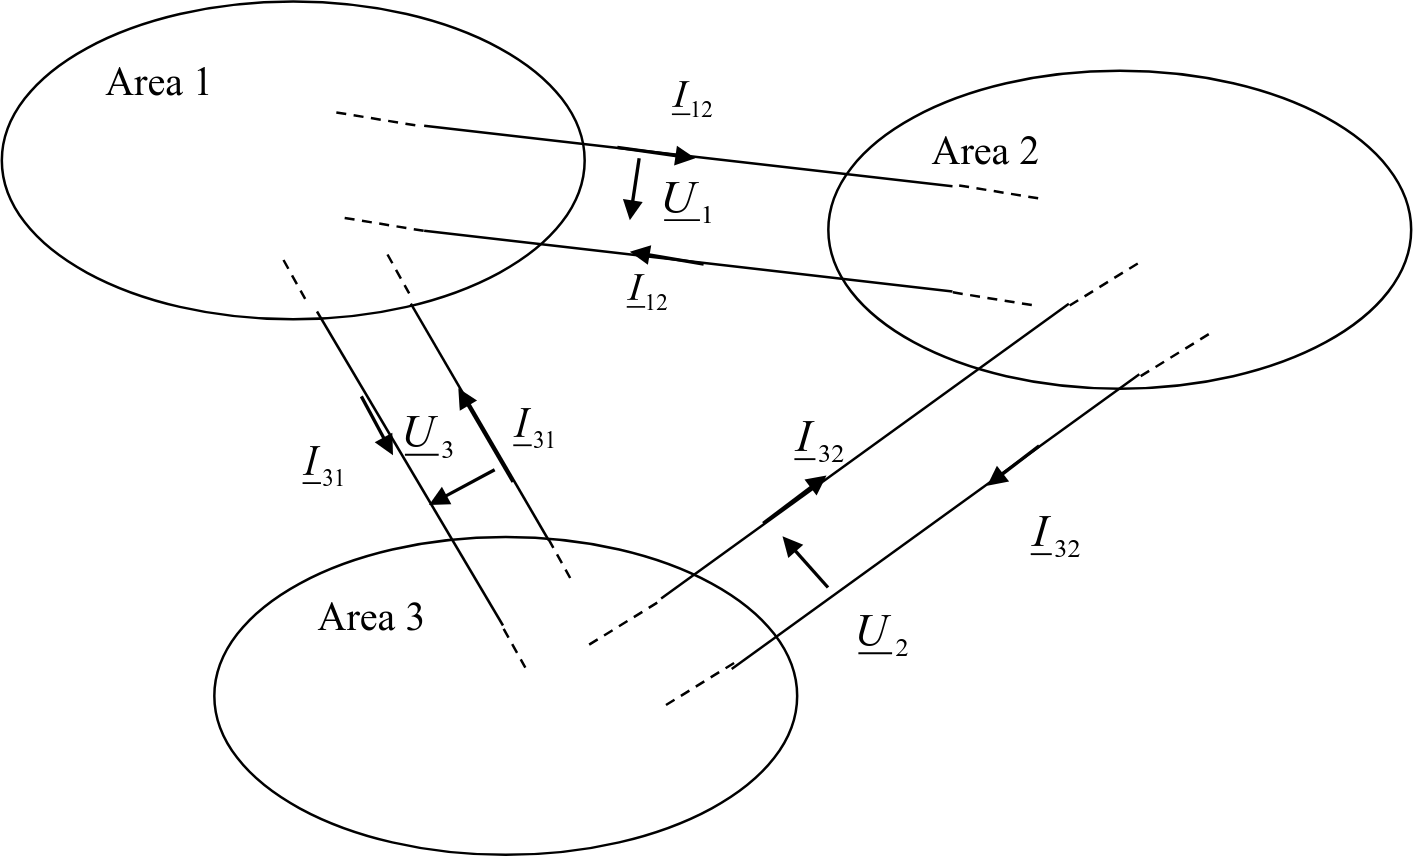
\includegraphics[\lw=.6]{media/ex1.png}
\end{center}
\begin{enumerate}
  \item Which areas provide active power? How much?
  \item Which areas receive reactive power? How much?
\end{enumerate}
\figbox{$\underline{S} = \underline{U}\cdot \underline{I}^* = \underline{U} + I \angle (-\theta^\circ)$}
\begin{align*}
  \underline{S}_1 &= \underline{U}_1 \underline{I}_{31}^*
  = 76\angle 4^\circ \cdot 450 \angle 15^\circ - 76\angle -11^\circ \cdot 300\angle -18^\circ\\
  &= 12.4 + j22.2\ [MW]\ = 12.4\ [MW]\ + 22.2\ [MVar]\\
  \underline{S}_2 &= \underline{U}_2\underline{I}_{32}^* - \underline{U}_1 \underline{I}_{12}^* = 3.59\ [MW]\ + j1.24\ [MVar]\\
  \underline{S}_3 &= \underline{U}_3\underline{I}_{31}^* - \underline{U}_2 \underline{I}_{32}^* = -15.99\ [MW]\ - j23.43\ [MVar]
\end{align*}
Conventionally, $S,Q > 0$: provider,\ $S,Q < 0$: receiver
\begin{enumerate}
  \item $\underline{S}_1,2$: provider, 12.4 MW and 3.59 MW
  \item $\underline{S}_3$: receiver, 23.43 MVar
\end{enumerate}

\textbf{Exercise 2: Merit-order pricing}\\
Sorted list of B1--B6 consumer offers:
\vspace*{-.4cm}
\begin{center}
\renewcommand{\arraystretch}{1.3}
\resizebox{\columnwidth}{!}{%
\begin{tabular}{|c|c|c|c|c|c|}
  \hline
  B1 & B2 & B3 & B4 & B5 & B6\\
  \hline
  \makecell{100 MWh\\0.08 Fr./kWh} &
  \makecell{200 MWh\\0.09 Fr./kWh} &
  \makecell{250 MWh\\0.10 Fr./kWh} &
  \makecell{250 MWh\\0.11 Fr./kWh} &
  \makecell{150 MWh\\0.12 Fr./kWh} &
  \makecell{150 MWh\\0.13 Fr./kWh}\\
  \hline
\end{tabular}%
}
\end{center}

Sorted list of offers of electricity sellers S1--S5:
\vspace*{-.4cm}
\begin{center}
\renewcommand{\arraystretch}{1.3}
\resizebox{\columnwidth}{!}{%
\begin{tabular}{|c|c|c|c|c|}
  \hline
  S1 & S2 & S3 & S4 & S5\\
  \hline
  \makecell{50 MWh\\0.07 Fr./kWh} &
  \makecell{200 MWh\\0.075 Fr./kWh} &
  \makecell{250 MWh\\0.085 Fr./kWh} &
  \makecell{250 MWh\\0.095 Fr./kWh} &
  \makecell{400 MWh\\0.15 Fr./kWh}\\
  \hline
\end{tabular}%
}

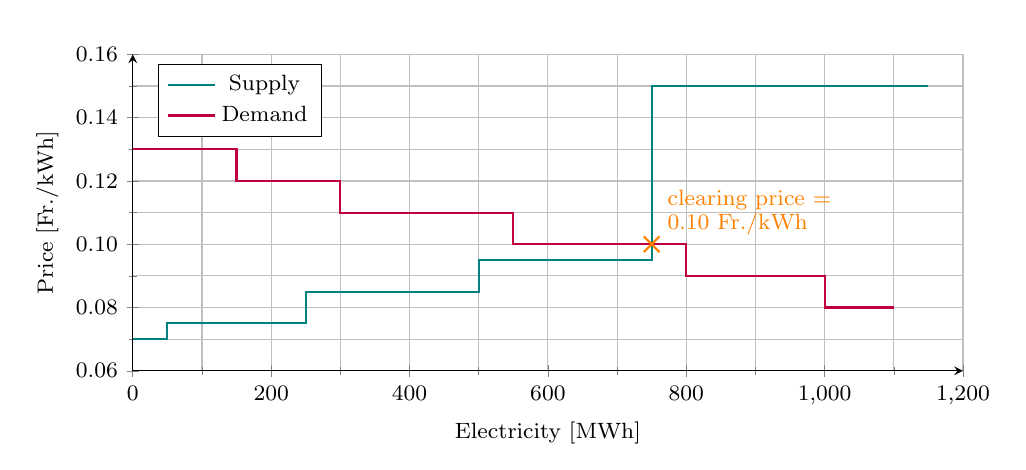
\begin{tikzpicture}
\begin{axis}[
    width=\linewidth,
    height=5.6cm,
    xmin=0, xmax=1200,
    ymin=0.06, ymax=0.16,
    xlabel={Electricity [MWh]},
    ylabel={Price [Fr./kWh]},
    xtick={0,200,400,600,800,1000,1200},
    ytick={0.06,0.08,0.10,0.12,0.14,0.16},
    scaled y ticks=false,
    y tick label style={
        /pgf/number format/fixed,
        /pgf/number format/precision=2,
        /pgf/number format/fixed zerofill,
    },
    grid=both,
    minor tick num=1,
    axis lines=left,
    legend pos=north west,
    legend style={font=\footnotesize},
    tick label style={font=\footnotesize},
    label style={font=\footnotesize},
]

% Supply curve: sellers S1--S5
\addplot[
    const plot,
    thick,
    teal,
] coordinates {
    (0,0.070)
    (50,0.075)
    (250,0.085)
    (500,0.095)
    (750,0.150)
    (1150,0.150)
};
\addlegendentry{Supply}

% Demand curve: consumers B6--B1
\addplot[
    const plot,
    thick,
    purple,
] coordinates {
    (0,0.130)
    (150,0.120)
    (300,0.110)
    (550,0.100)
    (800,0.090)
    (1000,0.080)
    (1100,0.080)
};
\addlegendentry{Demand}

% Clearing price
\addplot[
    only marks,
    mark=x,
    mark size=4pt,
    thick,
    orange,
] coordinates {(750,0.100)};

\node[anchor=south west, font=\footnotesize, orange]
    at (axis cs:760,0.108) {clearing price =};
\node[anchor=south west, font=\footnotesize, orange]
    at (axis cs:760,0.100) {0.10 Fr./kWh};

\end{axis}
\end{tikzpicture}
\end{center}

\textbf{Exercise 3: Three-phase power}
\begin{center}
  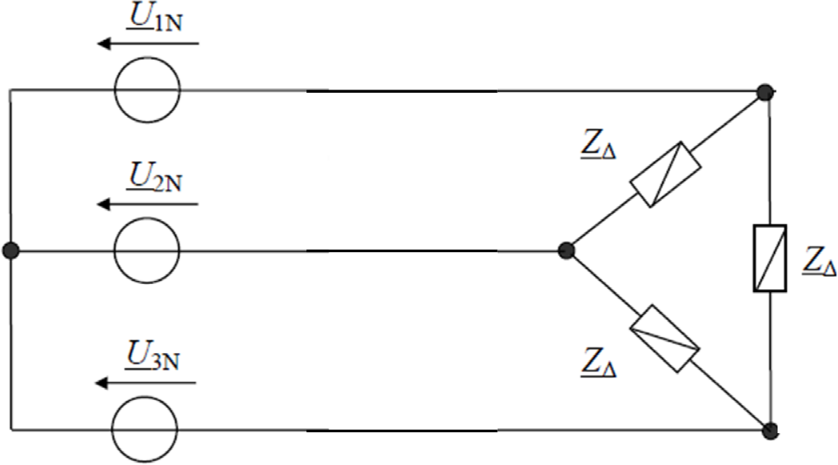
\includegraphics[\lw=.6]{media/ex3.png}
\end{center}
\underline{Data}:
\begin{gather*}
  \underline{U}_{1N} = 110\,\mathrm{V}\angle 0^\circ, \qquad
  \underline{U}_{2N} = 230\,\mathrm{V}\angle -120^\circ, \qquad
  \underline{U}_{3N} = 230\,\mathrm{V}\angle 120^\circ,\\
  \underline{Z}_{\Delta} = (30 + j25)\,\Omega
\end{gather*}
Calculate the complex power $\underline{S}$ and the power factor $\underline{\lambda}$
\figbox{$\underline{S} = \dfrac{\sum_i\left|\underline{U}\right|^2_i}{\underline{Z}_{\Delta}^{*}}$}
\begin{align*}
  \underline{U}_{12}
  &= \underline{U}_{1N} - \underline{U}_{2N}
  = 110\angle 0^\circ\,\mathrm{V} - 230\angle -120^\circ\,\mathrm{V}
  = 300.5\angle 41.52^\circ\,\mathrm{V}\\
  \underline{U}_{23}
  &= \underline{U}_{2N} - \underline{U}_{3N}
  = 230\angle -120^\circ\,\mathrm{V} - 230\angle 120^\circ\,\mathrm{V}
  = 398.5\angle -90^\circ\,\mathrm{V}\\
  \underline{U}_{31}
  &= \underline{U}_{3N} - \underline{U}_{1N}
  = 230\angle 120^\circ\,\mathrm{V} - 110\angle 0^\circ\,\mathrm{V}
  = 300.5\angle 138.48^\circ\,\mathrm{V}\\[1mm]
  \underline{S}
  &= \frac{\left|\underline{U}_{12}\right|^2
    + \left|\underline{U}_{23}\right|^2
    + \left|\underline{U}_{31}\right|^2}
    {\underline{Z}_{\Delta}^{*}}
    = \frac{(300.5\,\mathrm{V})^2 + (300.5\,\mathrm{V})^2
    + (398.5\,\mathrm{V})^2}
    {39.05\angle -39.81^\circ\,\Omega}\\
  &= 6.68 + j5.56\,\mathrm{kVA}
  = 8.69\angle 39.81^\circ\,\mathrm{kW}\\
  \lambda &= \cos(39.81^\circ) = 0.768
\end{align*}

\textbf{Exercise 4: 4-wire system}
\begin{center}
  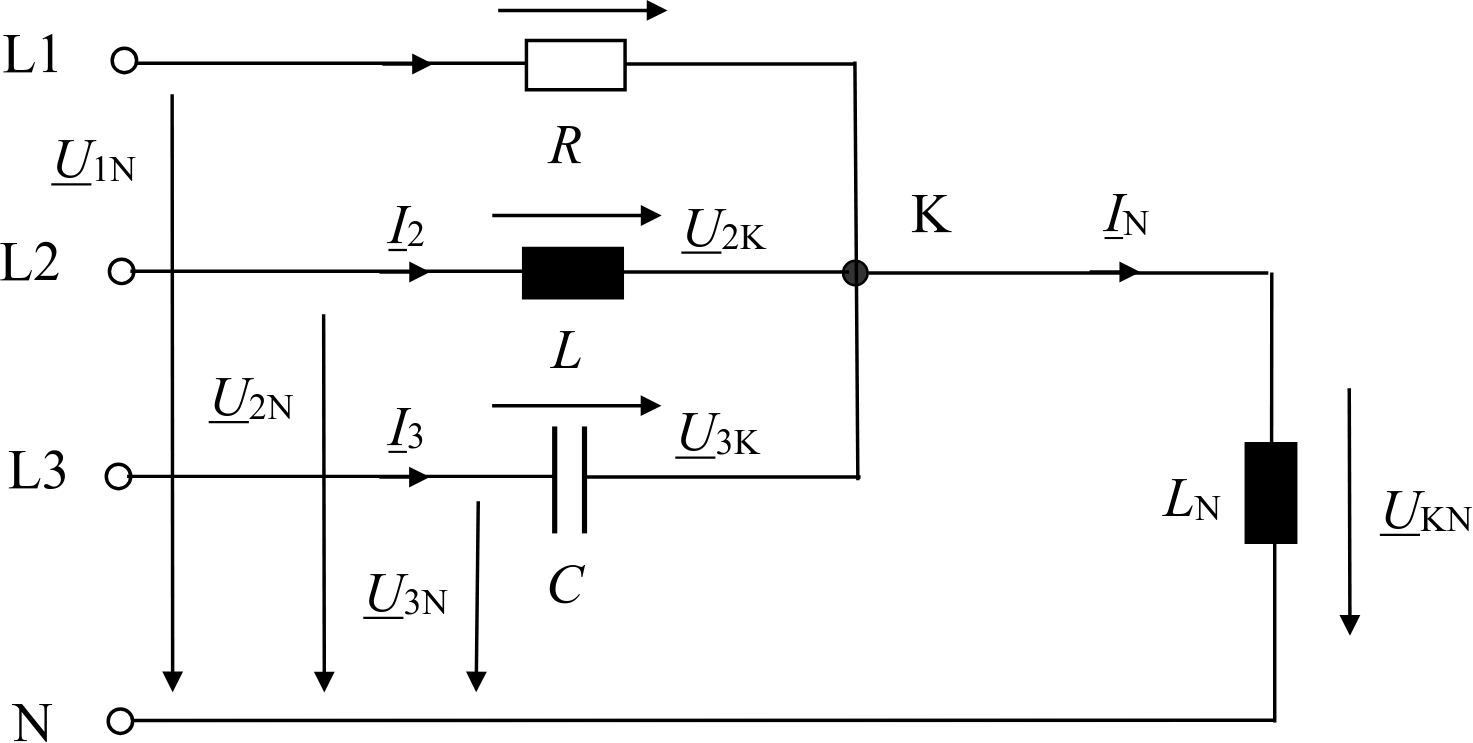
\includegraphics[\lw=.65]{media/ex4}
\end{center}
\underline{Data}:
\[
\begin{aligned}
  \underline{U}_{1N} &= 220\,\mathrm{V}\angle 0^\circ,
  &\qquad R &= 100\,\Omega,\\
  \underline{U}_{2N} &= 220\,\mathrm{V}\angle -120^\circ,
  & L &= 160\,\mathrm{mH},\\
  \underline{U}_{3N} &= 220\,\mathrm{V}\angle 120^\circ,
  & C &= 40\,\mu\mathrm{F},\\
  f &= 50\,\mathrm{Hz},
  & L_N &= 500\,\mathrm{mH}.
\end{aligned}
\]

Calculate: $\underline{I}_1$, $\underline{I}_2$, $\underline{I}_3$, $\underline{I}_N$, and
$\underline{U}_{1K}$, $\underline{U}_{2K}$, $\underline{U}_{3K}$, $\underline{U}_{KN}$.

\figbox{$\underline{U}_{KN} = \dfrac{\underline{Y}_1\underline{U}_{1N} + \underline{Y}_2\underline{U}_{2N} + \underline{Y}_3\underline{U}_{3N}}{\underline{Y}_1 + \underline{Y}_2 + \underline{Y}_3 + \underline{Y}_N}$\\[1.5ex]
        $\underline{U}_{iK} = \underline{U}_{iN}-\underline{U}_{KN}\quad ; \quad\underline{I}_i = \underline{U}_{iK}\cdot \underline{Y}_i$}

\newcolumn
\underline{Admittances}:\\[.5ex]
\noindent\(
\begin{aligned}
  \underline{Y}_1 = \underline{Y}_R
  &= \frac{1}{R}
  = 0.010\angle 0^\circ\,\mathrm{S},\\
  \underline{Y}_2 = \underline{Y}_L
  &= \frac{1}{\omega L}\angle -90^\circ
  = 0.0199\angle -90^\circ\,\mathrm{S},\\
  \underline{Y}_3 = \underline{Y}_C
  &= \omega C\angle 90^\circ
  = 0.0126\angle 90^\circ\,\mathrm{S},\\
  \underline{Y}_N = \underline{Y}_L
  &= \frac{1}{\omega L_N}\angle -90^\circ
  = 0.00637\angle -90^\circ\,\mathrm{S}.
\end{aligned}
\)

\underline{Voltages}:\\[.5ex]
\noindent\(
\begin{aligned}
  \underline{U}_{KN}
  &= \frac{\underline{Y}_1\underline{U}_{1N}
    + \underline{Y}_2\underline{U}_{2N}
    + \underline{Y}_3\underline{U}_{3N}}
    {\underline{Y}_1+\underline{Y}_2+\underline{Y}_3+\underline{Y}_N}
  = 238.4\angle -137.5^\circ\,\mathrm{V},\\[1mm]
  \underline{U}_{1K}
  &= \underline{U}_{1N}-\underline{U}_{KN}
  = 427.2\angle 22^\circ\,\mathrm{V},\\
  \underline{U}_{2K}
  &= \underline{U}_{2N}-\underline{U}_{KN}
  = 71.9\angle -24^\circ\,\mathrm{V},\\
  \underline{U}_{3K}
  &= \underline{U}_{3N}-\underline{U}_{KN}
  = 357.8\angle 79.4^\circ\,\mathrm{V}.
\end{aligned}
\)

\underline{Currents}:\\[.5ex]
\noindent\(
\begin{aligned}
  \underline{I}_1
  &= \underline{U}_{1K}\underline{Y}_1
  = 4.27\angle 22^\circ\,\mathrm{A},\\
  \underline{I}_2
  &= \underline{U}_{2K}\underline{Y}_2
  = 1.43\angle -114^\circ\,\mathrm{A},\\
  \underline{I}_3
  &= \underline{U}_{3K}\underline{Y}_3
  = 4.51\angle 169.4^\circ\,\mathrm{A},\\
  \underline{I}_N
  &= \underline{U}_{KN}\underline{Y}_N
  = 1.52\angle 132.5^\circ\,\mathrm{A}.
\end{aligned}
\)

\textbf{Exercise 5: Three-phase systems}
\begin{center}
  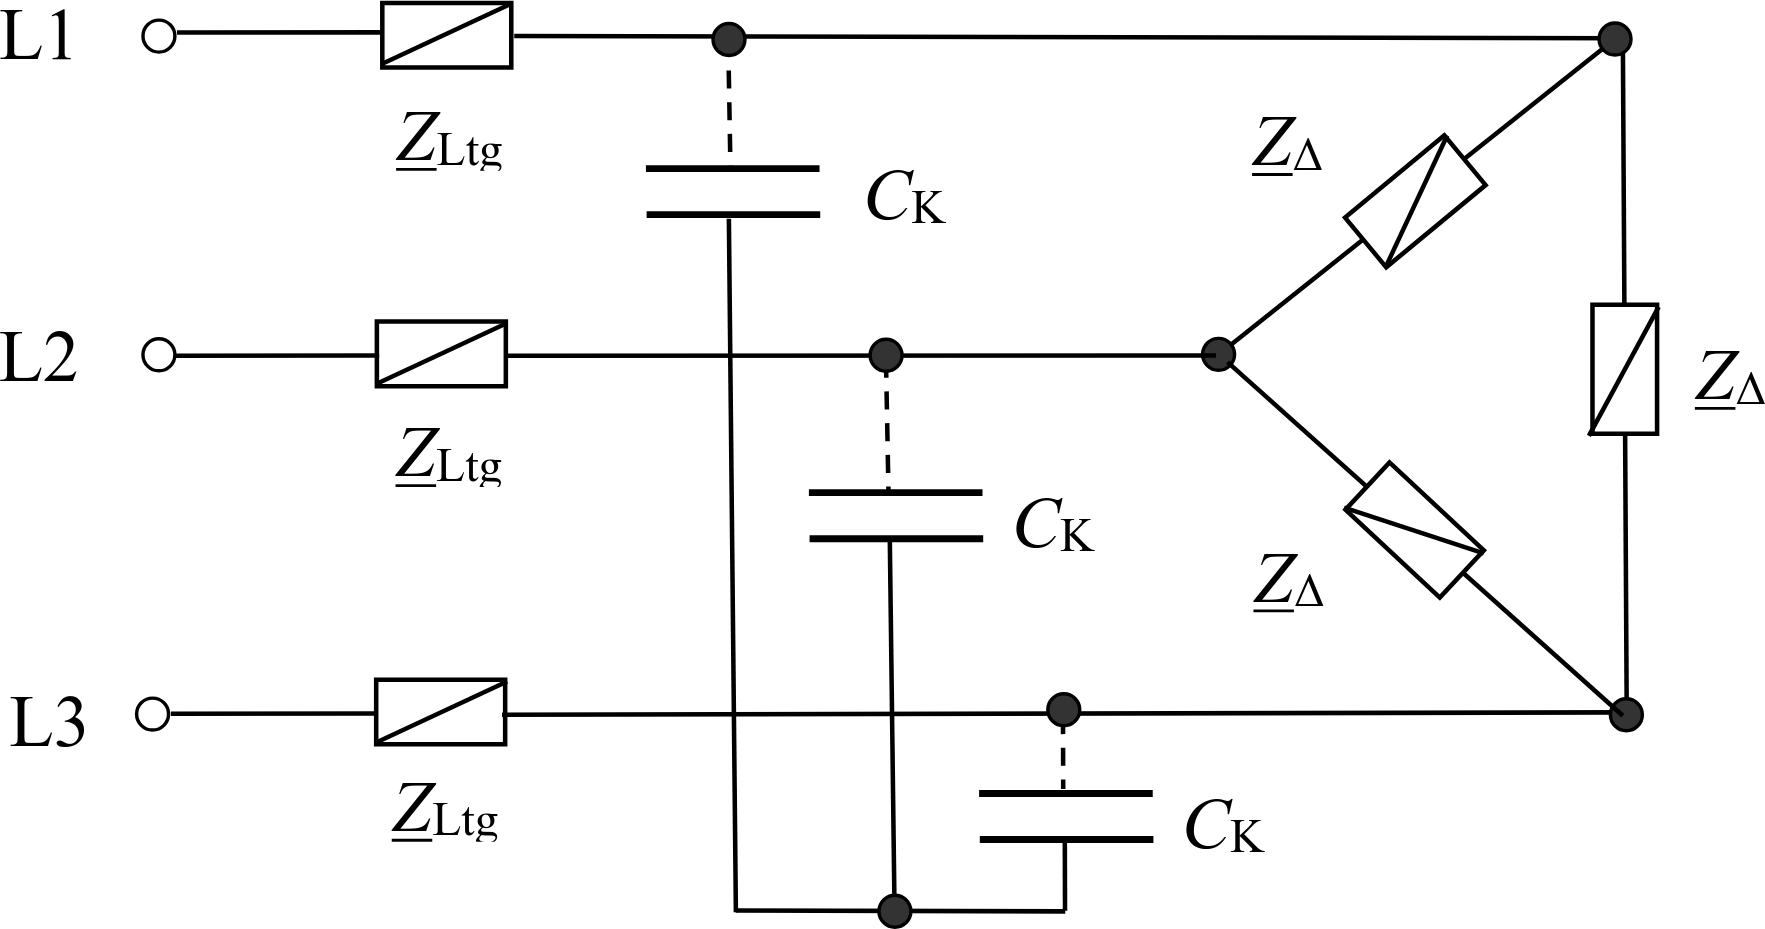
\includegraphics[\lw=.7]{media/ex5.png}
\end{center}
\underline{Data}:
\[U_\text{LL} = 400 V / 50 Hz\quad ; \quad\underline{Z}_\text{Ltg} = (1+j2) \Omega\quad ; \quad\underline{Z}_\Delta = 30\angle 60^\circ\]

\begin{enumerate}[label=\alph*)]
  \item Calculate the line currents $\underline{I}$ and the voltages
        $\underline{U}_{\Delta}$ across the loads $\underline{Z}_{\Delta}$
        without the capacitor bank connected.
  \item Calculate the capacitance $C_K$ of the capacitor bank for reactive
        current compensation of the loads $\underline{Z}_{\Delta}$.
  \item Determine the line currents $\underline{I}$ in the compensated case.
\end{enumerate}

\underline{a) Without compensation}:
\figbox{$\underline{I}_L = \dfrac{U_\text{ph}}{\underline{Z}_\text{Ltg} + \underline{Z}_Y} = \dfrac{\underline{U}_\text{LL}}{\sqrt{3}}\cdot \dfrac{1}{\underline{Z}_\text{Ltg} + \dfrac{\underline{Z}_\Delta}{3}}$\\[1ex]
        $\underline{U}_\Delta = \sqrt{3}\underline{U}_Y = \sqrt{3}\left(\underline{I}_L \underline{Z}_Y\right) = \sqrt{3}\left(\underline{I}_L\cdot \dfrac{\underline{Z}_\Delta}{3}\right)$}
\newcolumn
\(
  \underline{I}_1 = \dfrac{400 V}{\sqrt{3}}\cdot \dfrac{1}{(1+j2)\Omega + \dfrac{30\angle 60^\circ}{3}} = 18.88\angle -60.6^\circ A\\[1ex]
  \underline{I}_2 = \underline{I}_1 - 120^\circ = 18.88\angle 179.4^\circ\\[0.5ex]
  \underline{I}_3 = \underline{I}_1 + 120^\circ = 18.88\angle 59.4^\circ
\)

\(
  \underline{U}_\Delta = \sqrt{3}\left(18.88\angle -60.6^\circ \cdot \dfrac{30\angle 60^\circ}{3}\right) = 327 \angle -0.63^\circ\, [\mathrm{V}]
\)

\(
  \underline{U}_{12,\Delta} = \underline{U}_\Delta + 30^\circ = 327 \angle 29.7^\circ\, [\mathrm{V}]\\[0.5ex]
  \underline{U}_{23,\Delta} = \underline{U}_\Delta - 120^\circ = 327 \angle -90.63^\circ\, [\mathrm{V}]\\[0.5ex]
  \underline{U}_{31,\Delta} = \underline{U}_\Delta + 120^\circ = 327 \angle 149.37^\circ\, [\mathrm{V}]
\)

\(\underline{Z}_\Delta = \const\ = 30\angle 60^\circ \Omega\)

\underline{b) Compensation capacitance}:
\figbox{$\underline{Y}_C = j\omega C_k\quad ; \quad \underline{Y}_Y = \dfrac{1}{\underline{Z}_Y}\quad ; \quad \Im\left(Y_C + Y_Y\right) = 0$}
\(
  \underline{Y}_Y = \dfrac{3}{\underline{Z}_\Delta} = 0.05 - j0.0866\, \mathrm{S} \to \Im\left(\underline{Y}_Y\right) = -0.0866\, \mathrm{S}\\[0.5ex]
  \Im(\underline{Y}_C) = -\underline{Y}_Y = 0.0866\, \mathrm{S}\\[0.5ex]
  0.0866 = \omega C_k \Longrightarrow C_k = \dfrac{0.0866}{2\pi\cdot 50\, \mathrm{Hz}} = 275.8\, [\mu\mathrm{F}]
\)

\underline{c) With compensation}:
\figbox{$Y_\text{load} = \Re(\underline{Y}_Y)\quad ; \quad Z_\text{load} = \dfrac{1}{Y_\text{load}}\quad ; \quad Z_\text{tot} = Z_\text{load} + \underline{Z}_\text{Ltg}$}
\(
  \underline{Z}_\text{tot} = 20 \Omega + (1 + j2) \Omega = 21 + j2 \Omega
\)

\(
  \underline{I}_L = \dfrac{\underline{U}_\text{LL}}{\underline{Z}_\text{tot}} \to \underline{I}_1 = \dfrac{400\, [\mathrm{V}]}{\sqrt{3}}\cdot \dfrac{1}{21+j2 \Omega} = 10.95\angle -5.44^\circ\, [\mathrm{A}]\\[1ex]
  \underline{I}_2 = \underline{I}_1 - 120^\circ = 10.95\angle -125.44\, [\mathrm{A}]\\[0.5ex]
  \underline{I}_3 = \underline{I}_1 + 120^\circ = 10.95\angle 114.56\, [\mathrm{A}]
\)

\textbf{Exercise 6: Surge impedance loading}\\
Equivalent line model of a lossless line with load $R_L$:
\begin{center}
  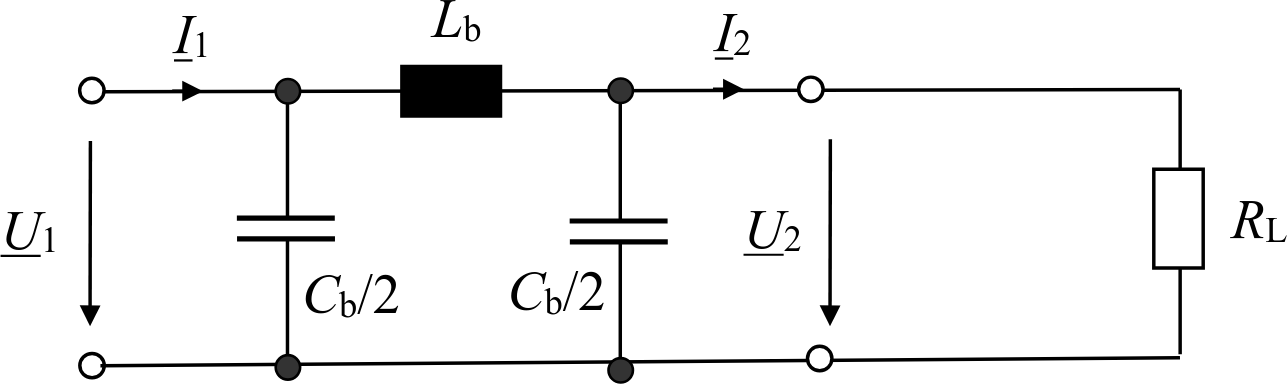
\includegraphics[\lw=.7]{media/ex6.png}
\end{center}
Determine $R_L$ so that the lossless line is optimal operation.
\underline{Data}:\\[.5ex]
\(
  L_b' = 1.3\, [\mathrm{mH}/\text{(km and phase)}]\quad ; \quad C_b' = 9.6\, [\mathrm{nF}/\text{(km and phase)}]\\[.5ex]
  l = 250\, [\mathrm{km} \text{( length of the line)}]
\)

\figbox{$Z_C = \sqrt{\dfrac{L_b'}{C_b'}} = \sqrt{\dfrac{L_b}{C_b}}\quad ; \quad L_b = L_b' \cdot l\quad ; \quad C_b = C_b' \cdot l$}

\(R_L = Z_C = \sqrt{\dfrac{\num[output-exponent-marker=\mathrm{E}]{1.3e-3}}{\num[output-exponent-marker=\mathrm{E}]{9.6e-9}}} = 368\, \Omega\)

\newcolumn
\textbf{Exercise 7: Transformers 1}
\begin{center}
  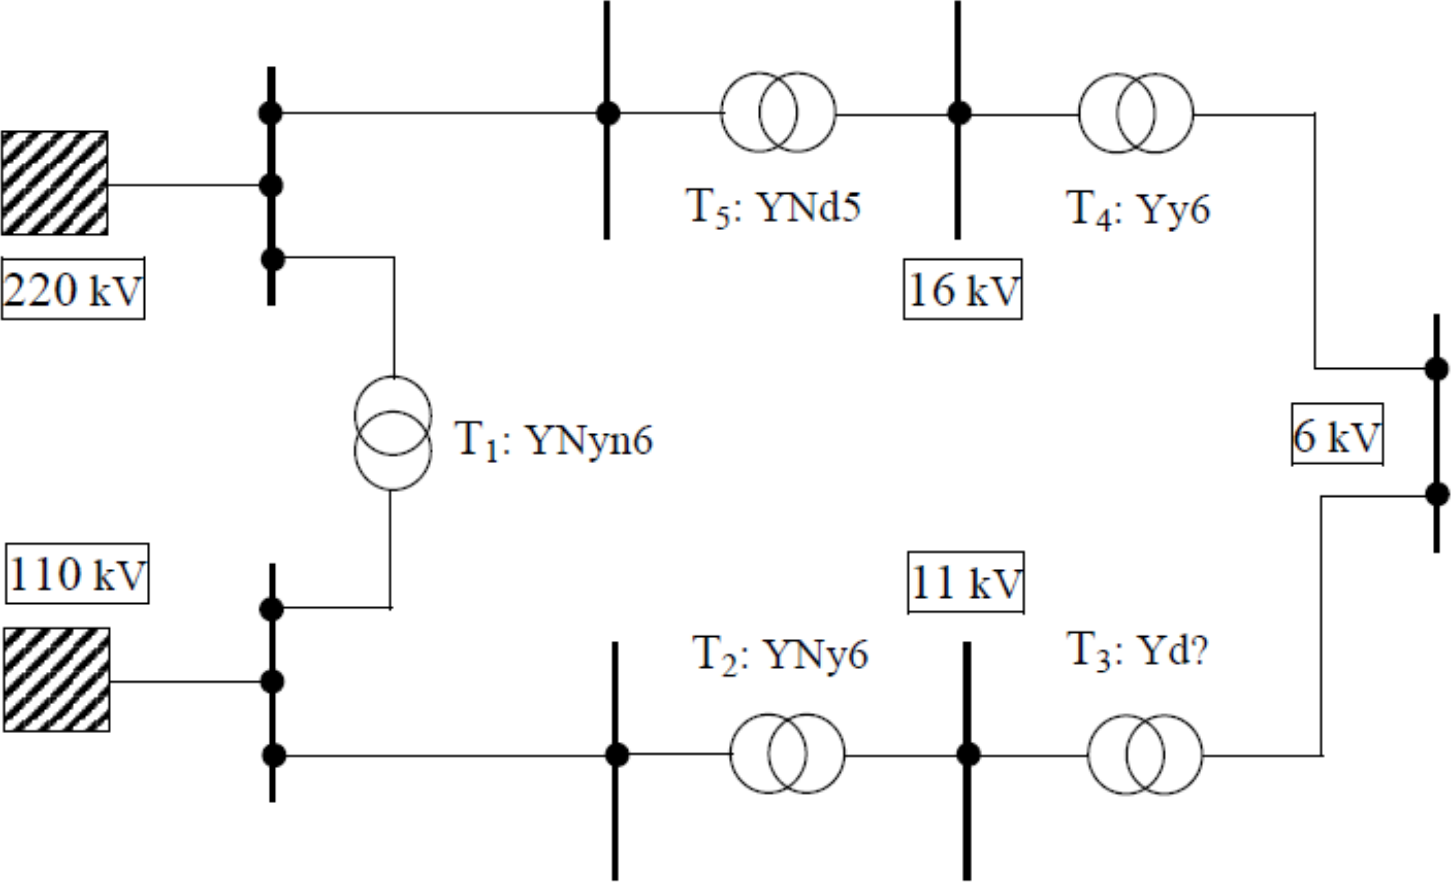
\includegraphics[\lw=.7]{media/ex7.png}
\end{center}
Determine the index number of transformer T$_3$.

\(
  \left(T5 + T4\right) \mod 12 = \left(T_3 + T_2 + T_1\right) \mod 12\\[.5ex]
  11 \mod 12 = (T_3 + 12) \mod 12\\[.5ex]
  \left(11-\cancel{12}\right) \mod 12 \equiv T_3 \to -1 \mod 12 \equiv T_3 \to T_3 = 11
\)

\textbf{Exercise 8: Transformer 2}
\begin{center}
  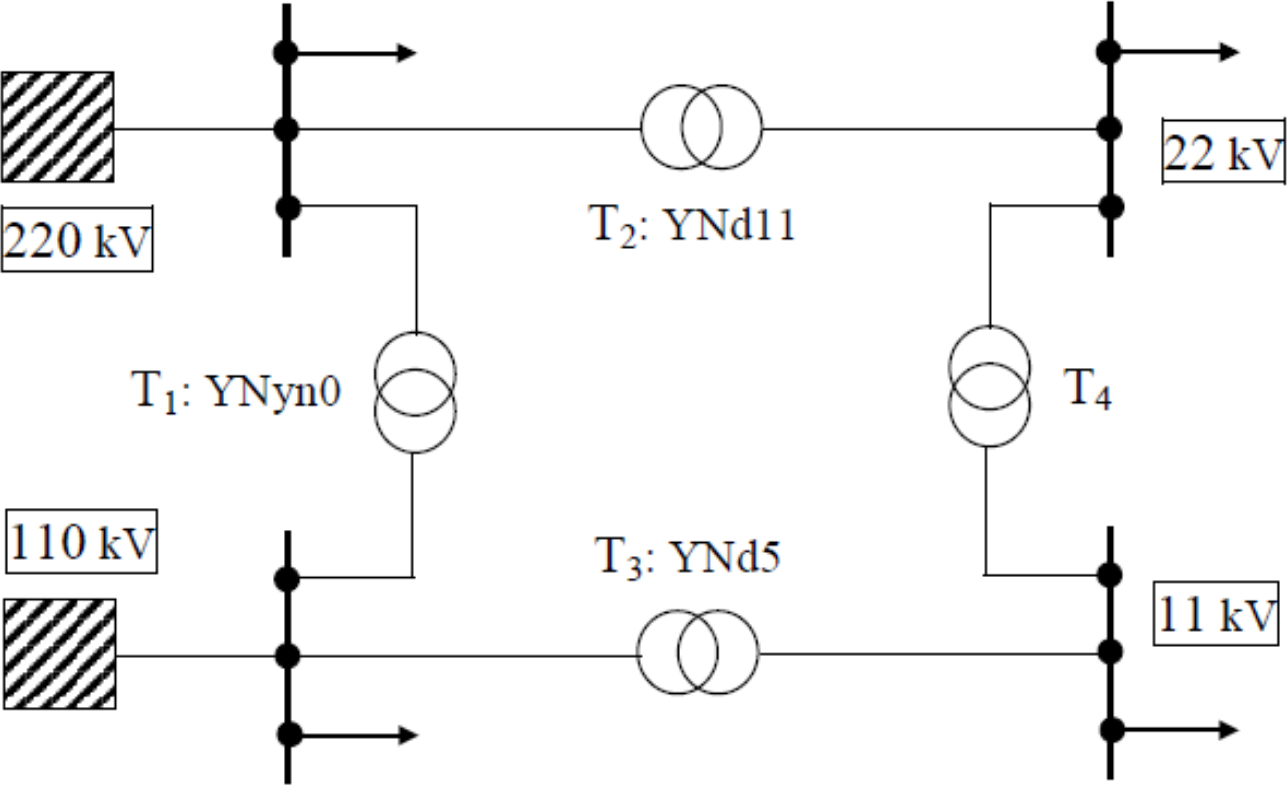
\includegraphics[\lw=.7]{media/ex8.png}
\end{center}
Determine a suitable transformer configuration for T$_4$.

\(
  T_2 + T_4 = T_3 + T_2 \Longrightarrow 11 + T_4 = 5\\[.5ex]
  11 + T_4 \equiv 5 \mod 12 \to T_4 = 6
\)

Suitable transformers: Dd6, Yy6, Dz6.

\textbf{Exercise 9: Active and reactive power of a synchronous generator}\\
A three-phase synchronous generator (star connected) is built as a nonsalient
pole machine. It operates at constant voltage and frequency.\\
\underline{Data}:\\
\(
  S_N=400\,\mathrm{MVA}\quad ; \quad U_N=20\,\mathrm{kV}\, /\, 50\, \mathrm{Hz}\quad ; \quad X_d=2\,\mathrm{p.u.}\\
  E=25\,\mathrm{kV}\quad ; \quad \delta=30^\circ
\)

$U_N$, unless otherwise specified, is line-to-line voltage.

Determine the active and reactive power of the generator.
Is the machine capacitive or inductive?

\figbox{$P = \dfrac{U\cdot U_p}{X_d}\sin(\vartheta)\quad ; \quad P_{3p} = 3\cdot P\\[1ex]
         Q = \dfrac{U\cdot U_p}{X_d}\cos(\vartheta) - \dfrac{U^2}{X_d}\quad ; \quad Q_{3p} = 3\cdot Q$}

\newcolumn
\(
  P = \dfrac{\num[output-exponent-marker=\mathrm{E}]{20e3}\, [\mathrm{V}]\cdot \num[output-exponent-marker=\mathrm{E}]{25e3}\, [\mathrm{V}]}{\sqrt{3}\cdot 2\, [\text{p.u.}]}\sin(30^\circ) = 72.2\, [\mathrm{MW}]\\[.5ex]
  P_{3p} = 3\cdot 72.2 = 216.6\, [\mathrm{MW}]
\)

\(
  Q = \dfrac{\num[output-exponent-marker=\mathrm{E}]{20e3}\, [\mathrm{V}]\cdot \num[output-exponent-marker=\mathrm{E}]{25e3}\, [\mathrm{V}]}{\sqrt{3}\cdot 2\, [\text{p.u.}]}\cos(30^\circ) - \dfrac{\left(\dfrac{\num[output-exponent-marker=\mathrm{E}]{20e3}\, [\mathrm{V}]}{\sqrt{3}}\right)^2}{2\, \text{p.u.}} = 58.33\, [\mathrm{MVA}]\\[.5ex]
  P_{3p} = 3\cdot 58.33 = 175\, [\mathrm{MVA}]
\)

\textbf{Exercise 10: Interconnected control areas}\\
Three control areas \(N_1\)--\(N_2\)--\(N_3\) are connected by \(L_1\) and
\(L_2\), initially without power exchange. A \(100\,\mathrm{MW}\) plant fails
in \(N_2\).

\(
  f_N=50\,\mathrm{Hz}\quad ; \quad K_{N1}=400\,\mathrm{MW/Hz}\quad ; \quad
  K_{N2}=K_{N3}=500\,\mathrm{MW/Hz}
\)

\begin{enumerate}[label=\alph*)]
  \item What frequency will occur in the control areas after the primary controllers have been activated?
  \item What power is then exchanged between the areas?
  \item What input signals $\Delta P_R$ are given to the secondary controllers of the three areas?
  \item When will the power exchange on L1 and L2 return to normal?
\end{enumerate}
\begin{center}
  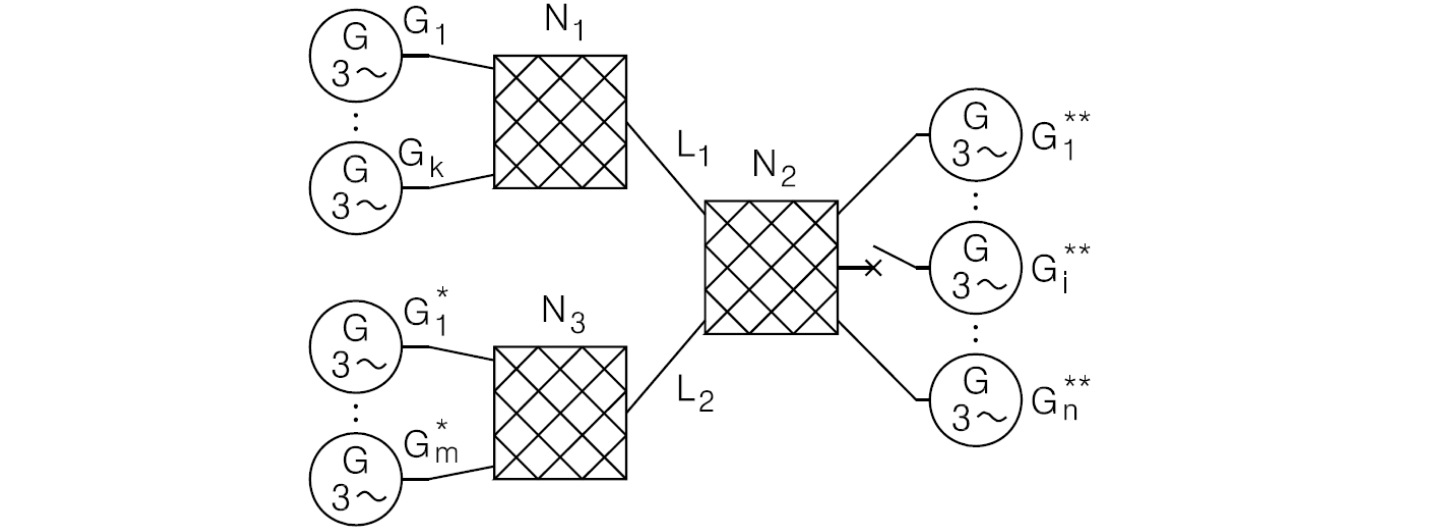
\includegraphics[\lw]{media/ex10.png}
\end{center}

\underline{a) Frequency shift}:
\figbox{$\Delta P_i = -\sum_i \left(K_{Ni}\right) \Delta f \Longleftrightarrow \Delta f = \dfrac{\Delta P}{-\left(\sum_i K_{Ni}\right)} $}
\(\Delta f = \dfrac{100\, [\mathrm{MW}]}{-\left(400+500+500\right)\, [\mathrm{MW/Hz}]} = -0.0714\, [\mathrm{Hz}]\)

\underline{b) Power exchanged}:
\figbox{$\Delta P_i = -K_{Ni} \Delta f$}
\(
  \Delta P_1 = -400\, [\mathrm{MW/Hz}] \cdot (-0.0714)\, [\mathrm{Hz}] = 28.56\, [\mathrm{MW}]\\[1ex]
  \Delta P_2 = \Delta P_3 = -500\, [\mathrm{MW/Hz}] \cdot (-0.0714)\, [\mathrm{Hz}] = 35.7\, [\mathrm{MW}]
\)

\underline{c) Secondary controllers}:
\figbox{$\Delta P_{Ri} = \Delta P_i - \Delta P_{Ki}$}
\(
  \Delta P_{R1} = \Delta P_1 + K_{N1}\Delta f = 28.56\, [\mathrm{MW}] - 28.56\, [\mathrm{MW}] = 0\, [\mathrm{MW}]\\[.5ex]
  \Delta P_{R2} = \Delta P_3 + K_{N3}\Delta f = 35.7\, [\mathrm{MW}] - 35.7\, [\mathrm{MW}] = 0\, [\mathrm{MW}]\\[.5ex]
  \Delta P_{R3} = \Delta P_2 + K_{N2}\Delta f = -\left(\Delta P_1 + \Delta P_3\right) + K_{N2}\Delta f\\[.5ex]
  \phantom{\Delta P_{R3}} = -(28.56 + 37.5)\, [\mathrm{MW}] + 500\cdot\left(-0.0714\right)\, [\mathrm{MW}] = -100\, [\mathrm{MW}]
\)

\underline{d) Time period}:
Between 5 to 15 minutes.

\newcolumn
\textbf{Exercise 11: Ybus}\\
Form the Ybus of the following system:
\begin{center}
  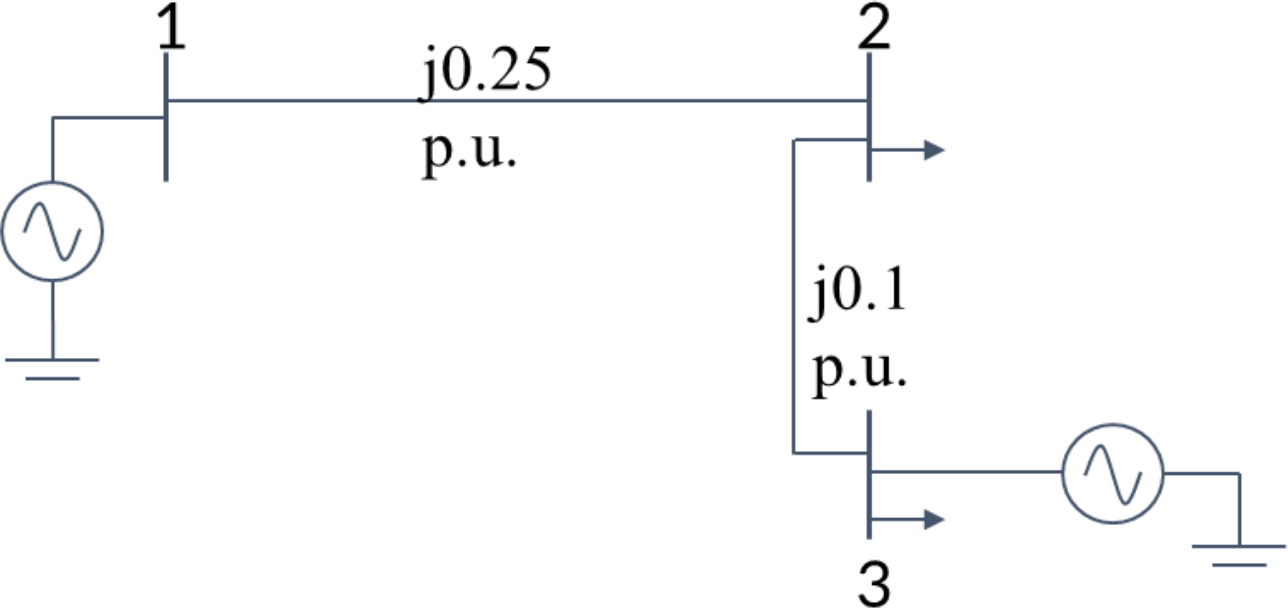
\includegraphics[\lw=.7]{media/ex11.png}
\end{center}
\(
  \begin{cases}
    I_1 = \dfrac{1}{j0.25}\left(v_1 - v_2\right)\\[2ex]
    I_2 = \dfrac{1}{j0.1}\left(v_2 - v_3\right) + \dfrac{1}{j0.25}\left(v_2 - v_1\right)\\[2ex]
    I_3 = \dfrac{1}{j0.1}\left(v_3 - v_2\right)
  \end{cases}
  \begin{cases}
    I_1 = -j4v_1 + j4v_2\\[2.5ex]
    I_2 = -j14v_2 + j10v_3 + j4v_1\\[2.5ex]
    I_3 = -j10v_3 + j10v_2
  \end{cases}
\)
\[
  \begin{bmatrix}
    I_1\\
    I_2\\
    I_3
  \end{bmatrix}
  =
  \begin{bmatrix}
    -j4 & j4 & 0\\
    j4 & -j14 & j10\\
    0 & j10 & -j10
  \end{bmatrix}
  \cdot
  \begin{bmatrix}
    v_1\\
    v_2\\
    v_3
  \end{bmatrix}
\]

\textbf{Exercise 12a: Two-node system ($P_B$ and $Q_B$)}
\begin{center}
  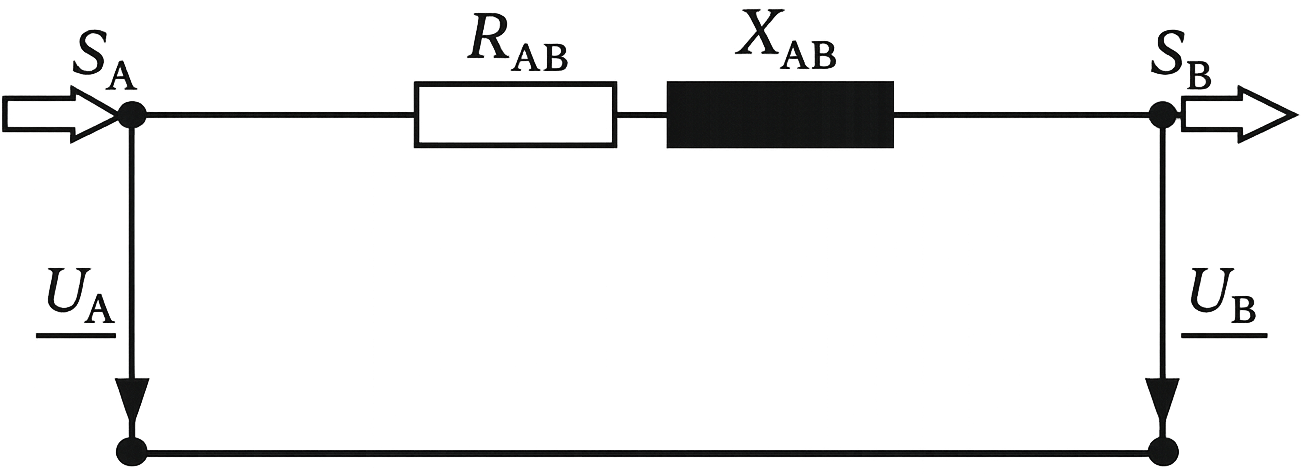
\includegraphics[\lw=.6]{media/ex12.png}
\end{center}
\underline{Data}:
\[
  \underline{U}_A = 400\angle0^\circ\, [\mathrm{V}],\quad Z_{AB} = 0.1 + j0.1\, [\Omega],\quad
  \underline{U}_B = 396.3\, e^{j(-0.1774^\circ)}\, [\mathrm{V}]
\]
Calculate $P_B$ and $Q_B$. Is the node inductive or capacitive?
\figbox{$Z_{AB} = R_{AB} + jX_{AB} = \left|Z_{AB}\right|e^{j\theta}$\\[1ex]
        $P_B = \dfrac{\left|U_A\right|\left|U_B\right|}{\left|Z_{AB}\right|}\cos(\theta + \delta) - \dfrac{\left|U_B\right|^2}{\left|Z_{AB}\right|}\cos(\theta)$\\[1ex]
        $Q_B = \dfrac{\left|U_A\right|\left|U_B\right|}{\left|Z_{AB}\right|}\sin(\theta + \delta) - \dfrac{\left|U_B\right|^2}{\left|Z_{AB}\right|}\sin(\theta)$
        }

\(
  Z_{AB} = 0.1414e^{j45^\circ}\, [\Omega]\\[.5ex]
  P_B = \dfrac{400\cdot396.3}{0.1414}\cos(45^\circ-0.1774^\circ)
  - \dfrac{396.3^2}{0.1414}\cos(45^\circ)
  = 9815\, [\mathrm{W}]\\[.5ex]
  Q_B = \dfrac{400\cdot396.3}{0.1414}\sin(45^\circ-0.1774^\circ)
  - \dfrac{396.3^2}{0.1414}\sin(45^\circ)
  = 4908\, [\mathrm{Var}]
\)

$Q_B > 0$ \to Node $B$ consumes reactive power \to Inductive system

\newcolumn
\textbf{Exercise 12b: Two-node system (Iterative process for $U_B$)}\\
\underline{Data}:
\[
  U_A = 400\, [\mathrm{V}]\ ; \ Z_{AB} = 0.1 + j0.1\, [\Omega]\ ; \
  P_B = 9815\, [\mathrm{W}]\ ; \ Q_B = 4908\, [\mathrm{Var}]
\]
Calculate $\underline{U}_B$ (magnitude and phase angle $\delta$).

\begin{enumerate}[label=Step \arabic*), itemsep=1.5ex]
  \item Initialize $i=0$ and $\underline{U}_B^{(0)}=\underline{U}_A$.
  \item Calculate the current:
        $\underline{I}_B^{(i)} =
        \left\{\dfrac{P_B+jQ_B}{\underline{U}_B^{(i)}}\right\}^*$.
  \item Update the voltage:
        $\underline{U}_B^{(i+1)} =
        \underline{U}_A-Z_{AB}\underline{I}_B^{(i)}$.
  \item Check convergence:
        $\left|\left|\underline{U}_B^{(i+1)}\right|
        -\left|\underline{U}_B^{(i)}\right|\right|<\varepsilon\ ;\ \varepsilon = \num[output-exponent-marker=\mathrm{E}]{1e-5}$.\\
        Otherwise, set $i=i+1$ and repeat from Step 2.
\end{enumerate}

\underline{Calculator iteration}:\\
Set $\mathrm{Ans}=\underline{U}_A$, then repeatedly enter
\figbox{\[
  \underline{U}_A-(Z_{AB})\,
  \dfrac{P_B-jQ_B}{\operatorname{CONJ}(\mathrm{Ans})}
\]}
until the result no longer changes. The final result is $\underline{U}_B$.

\underline{Result}:

$\underline{U}_B = 396.28\angle -0.18^\circ$ [V] $= 396.28 - j1.23$ [V]

\textbf{Exercise 13: Short circuits}
\begin{center}
  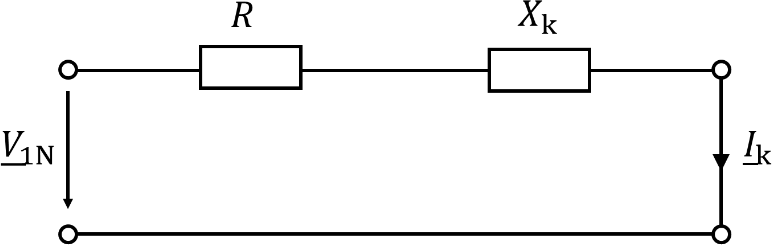
\includegraphics[\lw=.7]{media/ex13.png}
\end{center}
\underline{Data}:
\[V_L = 20\, [\mathrm{kV}]\quad ; \quad f = 50\, [\mathrm{Hz}]\quad ; \quad I_k = 300\, [\mathrm{A}]\quad ; \quad R = 12\, [\Omega]\]
\begin{enumerate}[label=\alph*)]
  \item Determine the value of the leakage reactance $X_k$
  \item Calculate the short-circuit current at time $t=0.03$ s.\\
        Assume that the short occurred at $t=0$ s.
\end{enumerate}
\figbox{$i(t) = i_s(t) + i_t(t)$\\[1.5ex]
        $i_s(t) = \dfrac{\sqrt{2}V_S}{\left|Z\right|}\sin(\omega t + \alpha - \Theta)$\\[1ex]
        $i_t(t) = -i_s(0)\cdot e^{-\left(R/L\right)t} = \dfrac{\sqrt{2}V_S}{\left|Z\right|}\sin\left(\Theta - \alpha\right)\cdot e^{-(R/L)t}$\\[1ex]
        $\left|Z\right| = \sqrt{R^2 + \omega^2L^2}\angle \left(\Theta = \tan^{-1}\left(\dfrac{\omega L}{R}\right)\right)$
}

\newcolumn
\underline{a) Leakage reactance}:

\(
  V_{1N} = \dfrac{V_L}{\sqrt{3}}\quad ; \quad I_k = \dfrac{V_{1N}}{\left|Z\right|} \Longrightarrow \left|Z\right| = \dfrac{V_L}{\sqrt{3}I_k}\\[.5ex]
  \left|Z\right| = \sqrt{R^2 + X_k^2} \Longrightarrow X_k = \sqrt{\left|Z\right|^2 - R^2} = \sqrt{\left(\dfrac{V_L}{\sqrt{3}I_k}\right)^2 - R^2}\\[.5ex]
  \phantom{\left|Z\right|} = \sqrt{\left(\dfrac{\num[output-exponent-marker=\mathrm{E}]{20e3}\, [\mathrm{V}]}{\sqrt{3}\cdot 300\, [\mathrm{A}]}\right)^2 - \left(12\, [\Omega]\right)^2} = 36.57\, [\Omega]
\)

\underline{b) Short circuit}:

$X_k = 2\pi f K \Longrightarrow K = \dfrac{X_k}{2\pi f} = \dfrac{36.57\, [\Omega]}{2\pi \cdot 50\, [\mathrm{Hz}]} = 0.1164\, [\mathrm{H}]$

\begin{align*}
  i_t(0) &= -i_s(0)e^{-(R/K)t}\\[.5ex]
  i_t(0.03) &= \sqrt{2}I_k\sin(\Theta)e^{-(12/0.1164)\cdot0.03}\\[.5ex]
  &= \sqrt{2}I_k\sin\left(\arctan\left(\dfrac{X_k}{R}\right)\right)e^{-(12/0.1164)\cdot0.03}\\[.5ex]
  &= \sqrt{2}\cdot 300\, [\mathrm{A}] \sin\left(\arctan\left(\dfrac{36.57\, [\Omega]}{12\, [\Omega]}\right)\right)e^{-(12/0.1164)\cdot0.03}\\[.5ex]
  &= 18.29\, [\mathrm{A}]
\end{align*}

\begin{align*}
  i_s(0.03) &= \sqrt{2}I_k \sin\left(2\pi f \cdot 0.03\, [\mathrm{s}] - \arctan\left(\dfrac{X_k}{R}\right)\right)\\[.5ex]
  &= \sqrt{2}\cdot 300\, [\mathrm{A}] \sin\left(2\pi \cdot 50\, [\mathrm{Hz}] \cdot 0.03\, [\mathrm{s}] - \arctan\left(\dfrac{0.1164\, [\mathrm{H}]}{12\, [\Omega]}\right)\right)\\[.5ex]
  &= 403.12\, [\mathrm{A}]
\end{align*}

\(i(t) = i_t(t) + i_s(t) = 403.12\, [\mathrm{A}] + 18.29\, [\mathrm{A}] = 421.41\, [\mathrm{A}]\)

\newcolumn
\vspace*{-.5cm}
\part{SW 1: Introduction}
\section{Swiss grid levels}
\begin{tabularx}{\columnwidth}{@{}lX@{}}
  \toprule
  \textbf{Voltage} & \textbf{Role}\\
  \midrule
  220/380 kV & transmission and international interconnection\\
  $\sim110$ kV & sub-transmission, large generation/loads\\
  10--40 kV & regional distribution\\
  0.4 kV & local distribution and households\\
  \bottomrule
\end{tabularx}

\section{Choice of grid voltage}
\subsection{Transmission losses}
\[
  P_{\mathrm{trans}}=U_mI
  \quad ; \quad
  P_\Omega=RI^2
  =R\left(\frac{P_{\mathrm{trans}}}{U_m}\right)^2
\]
\[
  P_{\mathrm{trans}}=\sqrt{3}\,U_LI_L\cos\varphi
  \quad ; \quad
  P_\Omega=\frac{P_{\mathrm{trans}}^2R}
  {U_L^2\cos^2\varphi}
\]
where: $P_{\mathrm{trans}}$ = transmitted active power; $P_\Omega$ =
resistive loss; $U_L$ = line-to-line RMS voltage.

\subsection{Economic optimum}
\begin{center}
  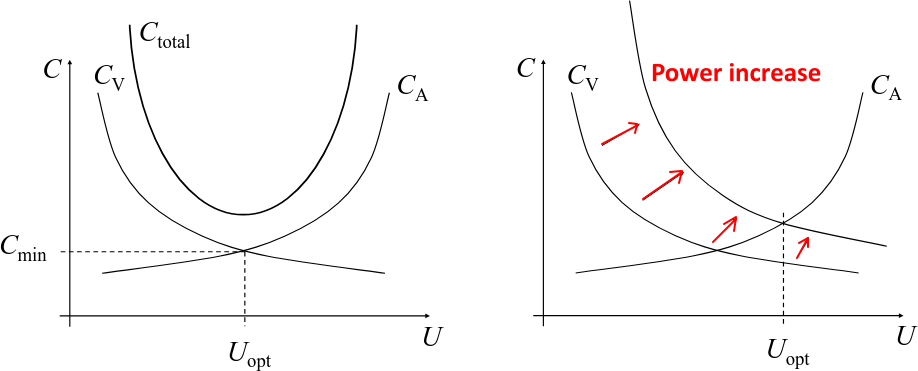
\includegraphics[\lw=.7]{media/economics.png}
\end{center}
\[
  C_{\mathrm{total}}=C_V+C_A
\]
where: $C_V$ = transmission-loss cost; $C_A$ = insulation/infrastructure
cost. \textbf{Rule of thumb}: economical transmission requires $\sim1$ kV/km.

\section{Reliability}
\textbf{$N-1$ criterion}: after any single component failure, the remaining
system continues operating without a system-wide outage.

\textbf{SAIDI}: average duration of long interruptions per customer and year
[min/(customer$\cdot$year)].

\section{Electricity markets}
\begin{itemize}
  \item \textbf{TSO}: secure transmission-system operation; CH: Swissgrid
  \item \textbf{Balance group}: financially responsible for deviations between
        scheduled and actual energy
  \item \textbf{Futures/OTC}: contracts before delivery
  \item \textbf{Day-ahead}: double auction for future delivery periods
  \item \textbf{Balancing}: TSO activation close to real time
\end{itemize}
\subsection{Merit order}
Offers are accepted from lowest to highest marginal cost until demand is met:
\[
  p_{\mathrm{market}}=\text{price of the last accepted offer}
\]

\newcolumn
\part{SW 2: Three-Phase Systems}
\section{AC elements and phasors}
\[
  U=\frac{\hat U}{\sqrt{2}}
  \quad ; \quad
  \omega=2\pi f
  \quad ; \quad
  \underline U=Ue^{j\varphi_u}=U\angle\varphi_u
\]
\[
  \frac{\mathrm d}{\mathrm dt}\longleftrightarrow j\omega
  \quad ; \quad
  \int\mathrm dt\longleftrightarrow\frac{1}{j\omega}
  \quad ; \quad
  \underline U=\underline Z\underline I
  \quad ; \quad
  \underline Y=\frac{1}{\underline Z}
\]
\begin{tabularx}{\columnwidth}{@{}lXX@{}}
  \toprule
  & \textbf{Impedance} & \textbf{Phase}\\
  \midrule
  R & $\underline Z_R=R$ & $u,i$ in phase\\
  C & $\underline Z_C=1/(j\omega C)$ & $i$ leads $u$ by $90^\circ$\\
  L & $\underline Z_L=j\omega L$ & $i$ lags $u$ by $90^\circ$\\
  \bottomrule
\end{tabularx}

\section{Complex power}
\[
  \underline S=\underline U\underline I^*=P+jQ
  \quad ; \quad
  S=UI=\sqrt{P^2+Q^2}
\]
\[
  P=UI\cos\varphi
  \quad ; \quad
  Q=UI\sin\varphi
  \quad ; \quad
  \lambda=\cos\varphi=\frac{P}{S}
\]
where: $\varphi=\varphi_u-\varphi_i$; $Q>0$ inductive/lagging; $Q<0$
capacitive/leading. Sign depends on the selected load/generator current
reference.

\section{Balanced three-phase systems}
\[
  \underline U_{1N}=U_{\mathrm{ph}}\angle0^\circ
  \quad ; \quad
  \underline U_{2N}=U_{\mathrm{ph}}\angle-120^\circ
  \quad ; \quad
  \underline U_{3N}=U_{\mathrm{ph}}\angle120^\circ
\]
\[
  \underline U_{12}=\underline U_{1N}-\underline U_{2N}
  =\sqrt{3}U_{\mathrm{ph}}\angle30^\circ
  \quad ; \quad
  U_{\mathrm{LL}}=\sqrt{3}U_{\mathrm{ph}}
\]

\section{Star and delta}
\begin{center}
  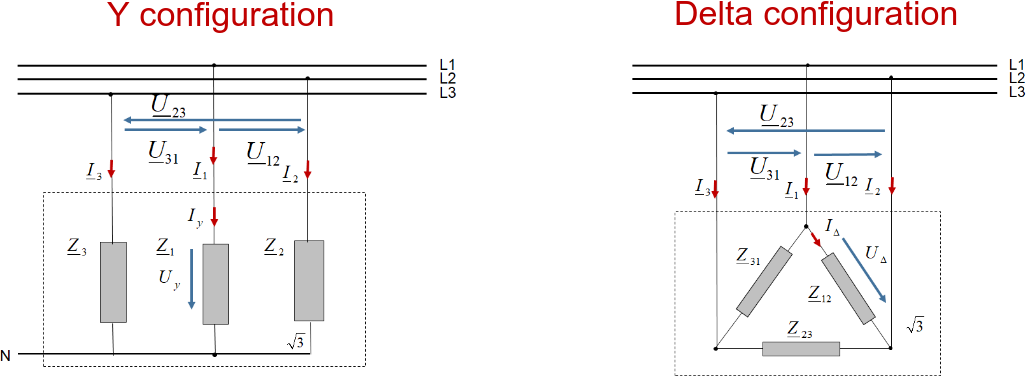
\includegraphics[\lw=.9]{media/star-delta-connections.png}
\end{center}
\[
  U_Y=\frac{U_{\mathrm{LL}}}{\sqrt3}
  \quad ; \quad I_Y=I_L
  \quad ; \quad U_\Delta=U_{\mathrm{LL}}
  \quad ; \quad I_\Delta=\frac{I_L}{\sqrt3}
\]
\[
  \underline Z_\Delta=3\underline Z_Y
  \quad ; \quad
  \underline Z_Y=\frac{\underline Z_\Delta}{3}
\]
Valid for balanced operation.

\section{Three-phase power}
\[
  \underline S_{3\mathrm{ph}}
  =3\underline U_{\mathrm{ph}}\underline I_{\mathrm{ph}}^*
  =\sqrt3\,U_{\mathrm{LL}}I_L\angle\varphi=P+jQ
\]
\[
  S=\sqrt3\,U_{\mathrm{LL}}I_L
  \quad ; \quad
  P=\sqrt3\,U_{\mathrm{LL}}I_L\cos\varphi
  \quad ; \quad
  Q=\sqrt3\,U_{\mathrm{LL}}I_L\sin\varphi
\]

\section{Unbalanced star loads}
\[
  \underline Y_i=\frac{1}{\underline Z_i}
\]
\subsection{Without neutral conductor}
\[
  \underline U_{KN}=
  \frac{\underline Y_1\underline U_{1N}
  +\underline Y_2\underline U_{2N}
  +\underline Y_3\underline U_{3N}}
  {\underline Y_1+\underline Y_2+\underline Y_3}
\]
\subsection{With neutral impedance}
\[
  \underline U_{KN}=
  \frac{\underline Y_1\underline U_{1N}
  +\underline Y_2\underline U_{2N}
  +\underline Y_3\underline U_{3N}}
  {\underline Y_1+\underline Y_2+\underline Y_3+\underline Y_N}
  \quad ; \quad
  \underline Y_N=\frac{1}{\underline Z_N}
\]
\[
  \underline U_{iK}=\underline U_{iN}-\underline U_{KN}
  \quad ; \quad
  \underline I_i=\underline Y_i\underline U_{iK}
  \quad ; \quad
  \underline I_N=\underline I_1+\underline I_2+\underline I_3
\]
Ideal neutral: $\underline Z_N=0\Longrightarrow\underline U_{KN}=0$.

\part{SW 3: Power Lines \& Transformers}
\section{Stiff grid}
Grid whose voltage magnitude $U$ and frequency $f$ remain approximately
constant independently of the connected load:
\[
  \Delta U\approx0
  \quad ; \quad
  \Delta f\approx0
\]
Equivalent to an ideal voltage source with very low internal impedance and high
short-circuit power.

\section{Equivalent line model}
\[
  R=R'l\quad ; \quad L=L'l
  \quad ; \quad G=G'l\quad ; \quad C=C'l
\]
\[
  \underline Z=(R'+j\omega L')l
  \quad ; \quad
  \underline Y=(G'+j\omega C')l
\]
\begin{center}
  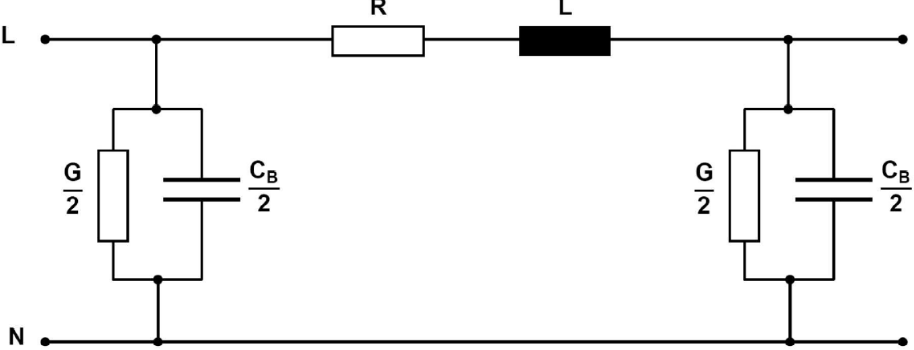
\includegraphics[\lw=.82]{media/line-pi-model.png}
\end{center}
\begin{tabularx}{\columnwidth}{@{}lXX@{}}
  \toprule
  \textbf{Length} & \textbf{Model} & \textbf{Elements}\\
  \midrule
  $<100$ km & short & series $\underline Z$\\
  100--300 km & medium & lumped $\Pi$\\
  $>300$ km & long & distributed / cascaded $\Pi$\\
  \bottomrule
\end{tabularx}

\subsection{Line parameters}
\[
  L'=\frac{\mu_0}{2\pi}\ln\left(\frac D{r'}\right)
  \quad ; \quad
  C'=\frac{2\pi\varepsilon\varepsilon_0}{\ln(D/r')}
  \quad ; \quad
  r'\approx0.78r
\]
\[
  R'_{\mathrm{DC}}=\frac{1}{\kappa A}
\]
where: $D$ = conductor spacing; $r$ = radius; $\kappa$ = conductivity.
$G'$ is often neglected.

\subsection{Skin effect}
AC-induced eddy currents reduce current density near the conductor centre:
\[
  \delta=\sqrt{\frac{2\rho}{\omega\mu}}
  =\sqrt{\frac{2}{\omega\mu\kappa}}
  \quad ; \quad
  R_{\mathrm{AC}}>R_{\mathrm{DC}}
\]
where: $\delta$ = penetration depth; at 50 Hz $\delta\approx9.38$ mm.

\section{Surge impedance loading}
\[
  Z_W=\sqrt{\frac{L'}{C'}}
\]
For $R'=G'=0$ and $Z_2=Z_W$:
\[
  Q_1=Q_2=0
  \quad ; \quad
  P_1=P_2=\frac{|U_1|^2}{Z_W}=\frac{|U_2|^2}{Z_W}
\]
Typical overhead line: $Z_W\approx200$--$400\,\Omega$.

\section{Voltage drop along a line}
\[
  \underline U_1=\underline U_2+jX\underline I_2
  \quad ; \quad
  \underline S_2=P_2+jQ_2=\underline U_2\underline I_2^*
\]
\[
  U_1\approx U_2+\frac{XQ_2}{U_2}
  \quad ; \quad
  \delta\approx\frac{XP_2}{U_2^2}
\]

\section{Transformers}
\subsection{Ideal and referred quantities}
\[
  \ddot u=\frac{N_1}{N_2}
  =\frac{\underline U_1}{\underline U_2}
  =\frac{\underline I_2}{\underline I_1}
  \quad ; \quad
  \underline S_1=\underline S_2
\]
\[
  \underline U'_2=\ddot u\,\underline U_2
  \quad ; \quad
  \underline I'_2=\frac{\underline I_2}{\ddot u}
  \quad ; \quad
  \underline Z'_2=\ddot u^{\,2}\underline Z_2
\]

\subsection{Equivalent circuit}
\begin{center}
  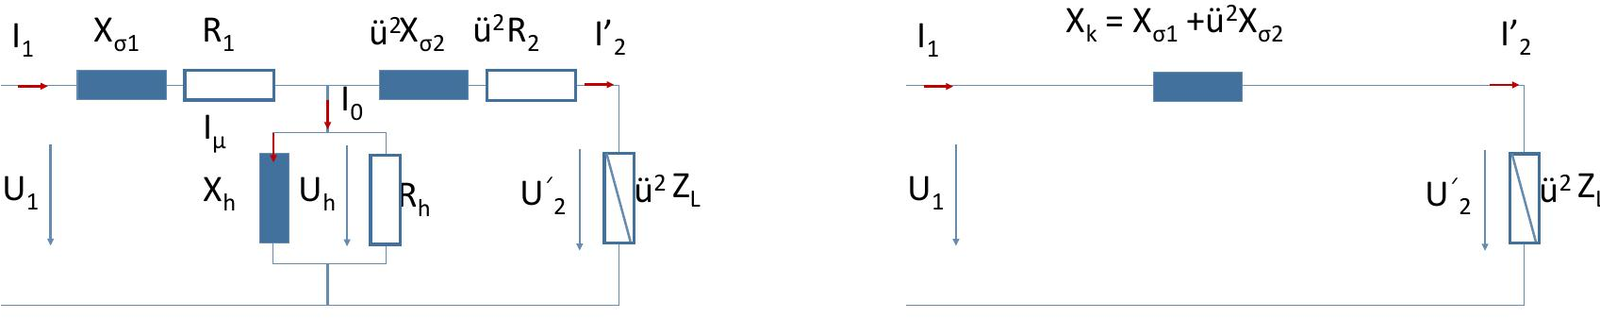
\includegraphics[\lw=.98]{media/transformer-equivalent-circuit.png}
\end{center}
\[
  R'_2=\ddot u^{\,2}R_2
  \quad ; \quad
  X'_{\sigma2}=\ddot u^{\,2}X_{\sigma2}
\]
\[
  R_k=R_1+R'_2
  \quad ; \quad
  X_k=X_{\sigma1}+X'_{\sigma2}
  \quad ; \quad
  \underline Z_k=R_k+jX_k
\]

\subsection{Relative short-circuit voltage}
\[
  u_k=\frac{U_{1k}}{U_{1N}}
  \quad ; \quad
  |\underline Z_k|=u_k\frac{U_N^2}{S_N}
\]
$u_k$: primary-voltage fraction producing nominal current with the secondary
short-circuited; typical range 4--18\%.

\section{Three-phase transformers}
\subsection{Connections and vector groups}
\begin{center}
  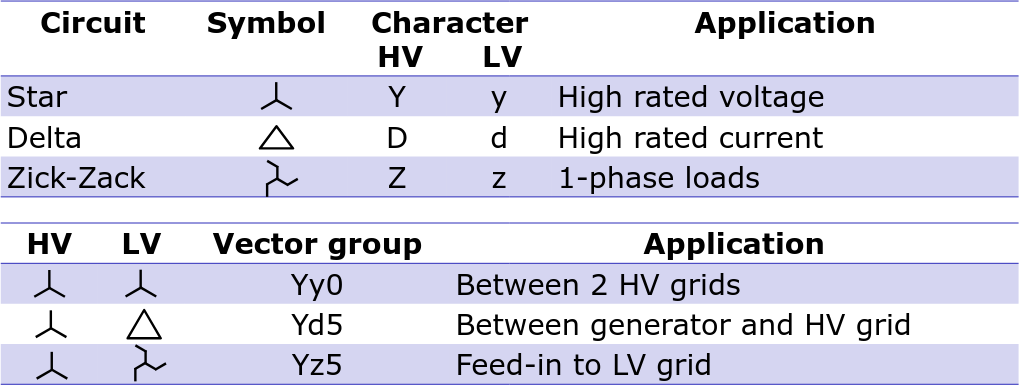
\includegraphics[\lw=.9]{media/transformers.png}
  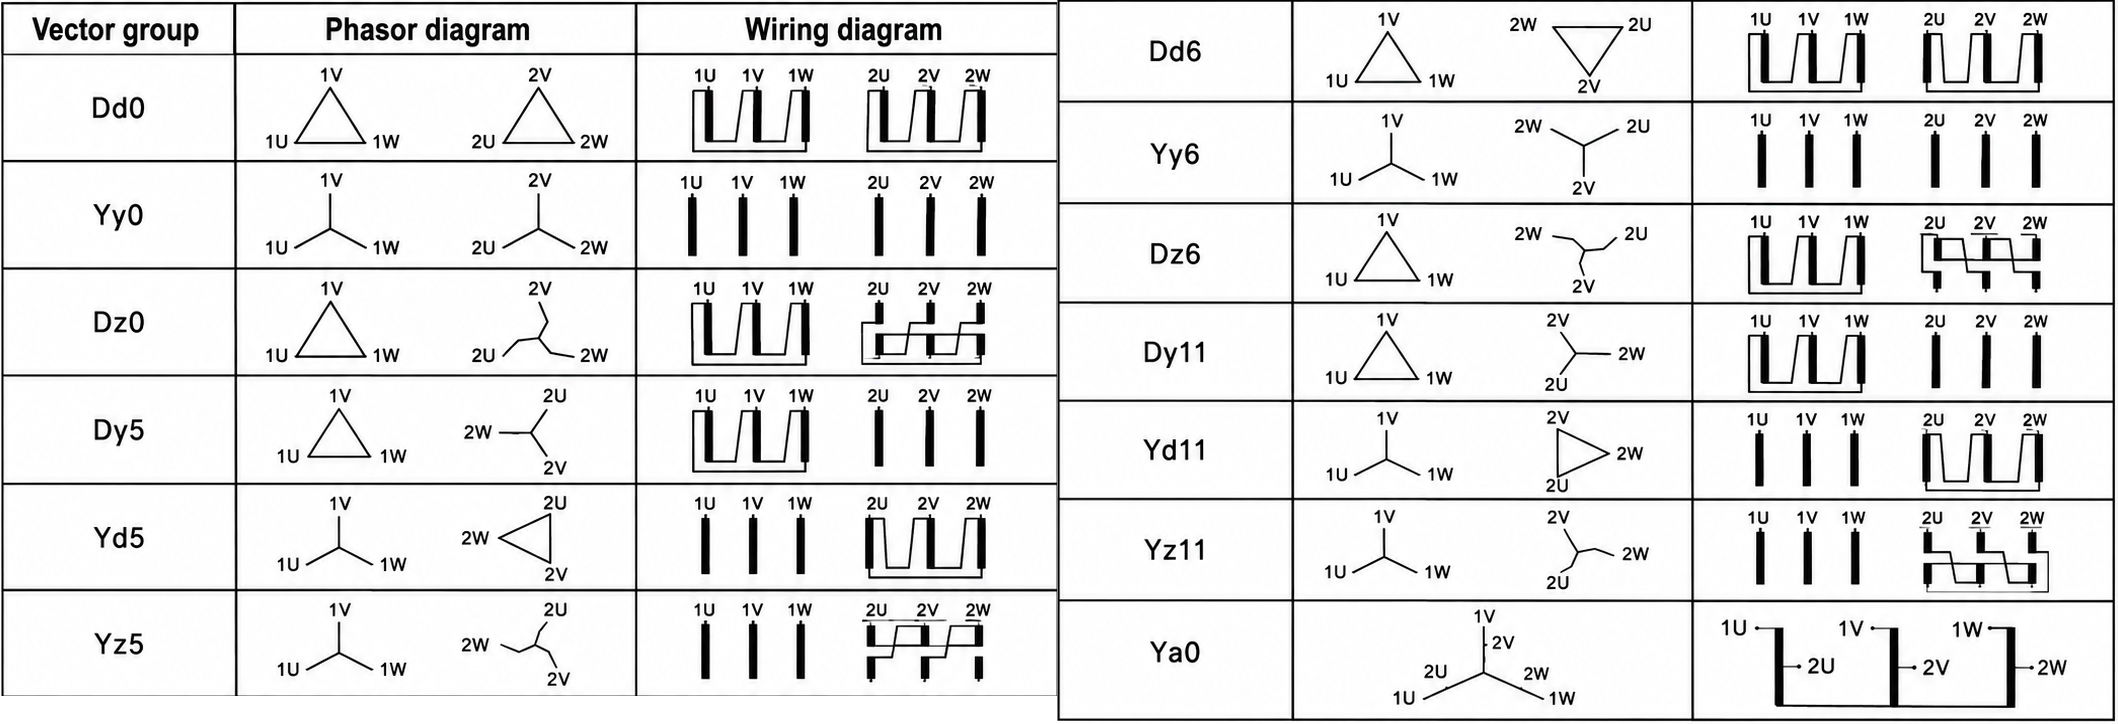
\includegraphics[\lw]{media/transformers2.png}
\end{center}
\[\underline{u} = \frac{\underline{U}_{OS}}{\underline{U}_{US}} = \frac{\underline{U}_{1U1V}}{\underline{U}_{2U2V}} = \frac{\underline{U}_{1U1N}}{\underline{U}_{2U2N}}\]

\newcolumn
\part{SW 4: Synchronous Generators}
\section{Three-phase generation}
A synchronous generator has a DC-excited or permanent-magnet rotor and three
stator windings displaced by $120^\circ$. The rotating magnetic field induces
three sinusoidal voltages.
\[
  U(t) = B\cdot A\cdot \omega\cdot \sin(\omega t)
  \quad ; \quad
  n=\frac{60f}{p}
  \quad ; \quad
  \omega_{\mathrm{mech}}=\frac{\omega}{p}=\frac{2\pi f}{p}=2\pi\frac{n}{60}
\]
where: $n$ = speed [rpm]; $p$ = number of pole pairs. Non-salient machines are
used at high speed; salient-pole machines use many poles for low-speed drives.

\subsection{Non-salient vs.\ salient-pole generators}
\begin{tabularx}{\columnwidth}{@{}lXX@{}}
  \toprule
  & \textbf{Non-salient pole} & \textbf{Salient pole}\\
  \midrule
  Rotor & cylindrical, nearly constant air gap & projecting poles, variable air gap\\
  Speed & high: typically 1500/3000 rpm & low: typically $\leq1000$ rpm\\
  Pole pairs & few: usually 1--2 & many\\
  Drive & steam/gas turbine & hydro turbine\\
  Model & $X_d=X_q$ & $X_d\neq X_q$\\
  \bottomrule
\end{tabularx}

\subsection{Grid inertia}
Rotating synchronous masses release kinetic energy after a power imbalance,
slowing the initial frequency change. Converter-based generation requires
synthetic/virtual inertia for the same function.

\section{Equivalent circuit and torque angle}
For stationary balanced operation of a non-salient generator, neglecting
stator resistance:
\begin{center}
  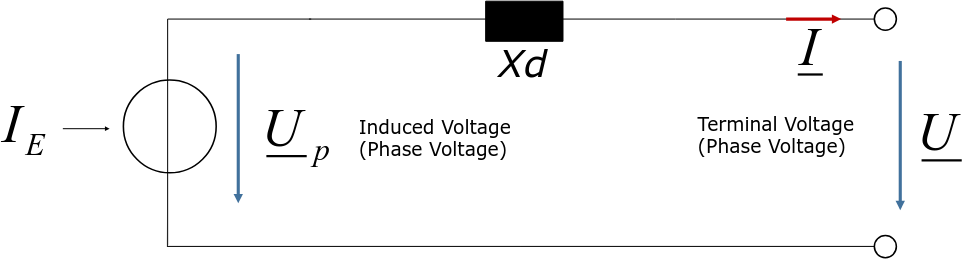
\includegraphics[\lw=.7]{media/synchronous-generator-equivalent.png}
\end{center}
\[
  X_d=X_m+X_\sigma
  \quad ; \quad
  \underline U_p=\underline U+jX_d\underline I
  \quad ; \quad
  \underline I=\frac{\underline U_p-\underline U}{jX_d}
\]
where: $\underline U_p$ = induced phase voltage; $\underline U$ = terminal
phase voltage; $X_d$ = synchronous reactance.
\[
  \vartheta=\varphi_{U_p}-\varphi_U
\]
$\vartheta>0$: generator operation; $\vartheta<0$: motor operation;
$\vartheta=0$: no active power.

\section{Active and reactive power}
With $\underline U=U\angle0^\circ$ and $\underline U_p=U_p\angle\vartheta$:
\[
  P=\frac{UU_p}{X_d}\sin\vartheta
  \quad ; \quad
  Q=\frac{UU_p}{X_d}\cos\vartheta-\frac{U^2}{X_d}
\]
\[
  P_{3\mathrm{ph}}=3P
  \quad ; \quad
  Q_{3\mathrm{ph}}=3Q
\]
\[
  P_{\max,3\mathrm{ph}}=\frac{3UU_p}{X_d}
  \quad\text{at}\quad \vartheta=90^\circ
\]

\section{Operating modes and excitation}
\begin{itemize}
  \item \textbf{Island operation}: excitation controls terminal voltage
  \item \textbf{Grid connected}: grid fixes $U$ and $f$; mechanical input mainly
        controls $P$, excitation mainly controls $Q$
  \item \textbf{Over-excited}: $U_p>U$, supplies $Q$ (capacitive behaviour)
  \item \textbf{Under-excited}: $U_p<U$, absorbs $Q$ (inductive behaviour)
\end{itemize}
At $\vartheta=0$:
\[
  P_{3\mathrm{ph}}=0
  \quad ; \quad
  Q_{3\mathrm{ph}}=\frac{3}{X_d}\left(U_pU-U^2\right)
\]

\section{Grid synchronization}
Connection to the grid requires:
\vspace*{-.2cm}
\begin{enumerate}[label=\arabic*.]
  \item equal frequency
  \item equal phase position
  \item equal voltage magnitude
  \item equal phase sequence L1--L2--L3
\end{enumerate}

\section{Per-unit system}
\subsection{Referenced quantities}
\[
  u=\frac{U}{U_N}
  \quad ; \quad
  i=\frac{I}{I_N}
  \quad ; \quad
  s=\frac{S}{S_N}
  \quad ; \quad
  z=\frac{Z}{Z_N}
\]
Per-unit values are dimensionless. Choose $U_N$ and $S_N$; the remaining base
values follow.

\subsection{Three-phase base values}
Using line-to-line $U_N$ and total three-phase $S_N$:
\[
  I_N=\frac{S_N}{\sqrt3\,U_N}
\]
\[
  Z_{N,Y}=\frac{U_N^2}{S_N}
  \quad ; \quad
  Z_{N,\Delta}=3\frac{U_N^2}{S_N}
\]
\[
  Z=zZ_N
\]
For the usual star-based network reference:
\[
  Z=z\frac{U_N^2}{S_N}
  \quad ; \quad
  z=Z\frac{S_N}{U_N^2}
\]


\end{multicols*}
\end{document}
